%%%%%%%%%%%%%%%%%%%%%%%%%%%%%%%%%%%%%%%%%%%%%%%%%%%%%%%%%%%%%%%%%%%%%%%%%%%%%%%%
% Template for USENIX papers.
%
% History:
%
% - TEMPLATE for Usenix papers, specifically to meet requirements of
%   USENIX '05. originally a template for producing IEEE-format
%   articles using LaTeX. written by Matthew Ward, CS Department,
%   Worcester Polytechnic Institute. adapted by David Beazley for his
%   excellent SWIG paper in Proceedings, Tcl 96. turned into a
%   smartass generic template by De Clarke, with thanks to both the
%   above pioneers. Use at your own risk. Complaints to /dev/null.
%   Make it two column with no page numbering, default is 10 point.
%
% - Munged by Fred Douglis <douglis@research.att.com> 10/97 to
%   separate the .sty file from the LaTeX source template, so that
%   people can more easily include the .sty file into an existing
%   document. Also changed to more closely follow the style guidelines
%   as represented by the Word sample file.
%
% - Note that since 2010, USENIX does not require endnotes. If you
%   want foot of page notes, do not include the endnotes package in the
%   usepackage command, below.
% - This version uses the latex2e styles, not the very ancient 2.09
%   stuff.
%
% - Updated July 2018: Text block size changed from 6.5" to 7"
%
% - Updated Dec 2018 for ATC'19:
%
%   * Revised text to pass HotCRP's auto-formatting check, with
%     hotcrp.settings.submission_form.body_font_size=10pt, and
%     hotcrp.settings.submission_form.line_height=12pt
%
%   * Switched from \endnote-s to \footnote-s to match Usenix's policy.
%
%   * \section* => \begin{abstract} ... \end{abstract}
%
%   * Make template self-contained in terms of bibtex entires, to allow
%     this file to be compiled. (And changing refs style to 'plain'.)
%
%   * Make template self-contained in terms of figures, to
%     allow this file to be compiled. 
%
%   * Added packages for hyperref, embedding fonts, and improving
%     appearance.
%   
%   * Removed outdated text.
%
%%%%%%%%%%%%%%%%%%%%%%%%%%%%%%%%%%%%%%%%%%%%%%%%%%%%%%%%%%%%%%%%%%%%%%%%%%%%%%%%

\documentclass[letterpaper,twocolumn,10pt]{article}
\usepackage{usenix2019_v3}

% to be able to draw some self-contained figs
\usepackage{tikz}
\usepackage{amsmath}

\usepackage{listings}
\usepackage{parcolumns}
\usepackage{graphicx}
\usepackage{caption}
\usepackage{subcaption}
\usepackage{cleveref}

% Comment macros
\newcommand{\pra}[1]{\textcolor{blue}{\textbf{PS:} #1}}
\newcommand{\nb}[1]{\textcolor{green}{\textbf{NB}: #1}}
\newcommand{\mat}[1]{\textcolor{red}{\textbf{Mat:} #1}}
%-------------------------------------------------------------------------------
\begin{document}
%-------------------------------------------------------------------------------

%do not want date printed
\date{}

% make title bold and 14 pt font (Latex default is non-bold, 16 pt)
\title{\Large \bf TikTok: Kernel TOCTTOU Protection}

%for single author (just remove % characters)
\author{
{\rm Eric Tusso}\\
EPFL
\and
{\rm Yamaha Priest}\\
EPFL
% copy the following lines to add more authors
% \and
% {\rm Name}\\
%Name Institution
} % end author

\maketitle

%-------------------------------------------------------------------------------
\begin{abstract}
%-------------------------------------------------------------------------------
We present TikTok - the first system that prevents double-fetch and
time-of-check-to-time-of-use (TOCTTOU) attack from user-space in system-calls. While dynamic and
static analysis techniques have focused on detecting and fixing double-fetch
bugs, TikTok focuses on mitigating them. This enables the use of the system-call
wrappers that can filter system-calls even on in-memory arguments. This wasn't
previously possible due to the unfixable TOCTTOU bug. System-call wrappers can
also benefit from TikTok's memory checkpointing system, which enables them to handle
system-calls that both read and write to user-memory.

% U.T. What else should be in the abstract? I know it has to be a sales pitch...

\end{abstract}
% Talk about the system call filters and how they can be used for good
% Introduce the main problem - TOCTTOU
% Brag how our system is the best thing since sliced bread
\section{Introduction}
% \nb{General notes: e.g. -> e.g., (as I've seen in all the hexhive papers\\
% privilige -> privilege\\
% userspace -> user space / user-space\\
% in .bib, title= should have double \{\{ brackets to keep capitalization tocttou
%   vs TOCTTOU\\
% in .bib, title= should have double \{\{ brackets to keep capitalization tocttou
%   vs TOCTTOU\\
% cref vs Cref\\
% -- vs --- (look at writing tips)}

%\mat{Start with one paragraph motivation/setting the scene.}

%\pra{You jump straight into introducing system call wrappers. Maybe preface
%this with a para detailing how system call execution model can be exploited in
%various scenarios. After that, you can jump into how wrappers try to address the
%problems you introduced first. It'd make for a smoother transition IMO.}


% \pra{I think the main message of the first paragraph should just be `syscalls are 
% vulnerable, adversaries can use them to to escalate privileges and hence
% is an attack surface that needs to be protected`. The last two points you make re:updates
% and drivers being distributed as binary blobs seem out of place. Give appropriate reasoning 
% as to why its relevant to your problem statement.}
% \pra{Additionally, a neat trick I learned from Mathias is to append a one-line
% description of the main message for each para as a comment (like presented below). 
% This not only helps you see the logical flow for each section but also helps a proofreader
% identify the main point you're trying to present in a para.}



%\pra{You introduce syscalls, say
%they are vulnerable. Then you switch to talking about update}
%\pra{Synonyms seem redundant and
%unnecessary. Just use one and stick with it throughout.} 

%\pra{Here this parenthesis makes me think you're
%implying kernel updates correspond to only kernel module updates which is not correct right?
%Updates can be pushed to core kernel components as well.}

% Syscalls are a lucrative attack surface for adversaries which needs to be protected
User space programs communicate with the operating system using system calls.
System calls may contain vulnerable code that a malicious user can exploit to
gain privileged access. Linux kernel contains hundreds of system calls and
can be extended by additional \texttt{ioctl} system calls that are part of
drivers. This amounts to a significant attack surface.

%\pra{Smoothen the transition to this para. Introduce syscall wrappers as a means to protect
%syscalls from exploitation.}

% Introduce wrappers and filters. Mention that they can be used to mitigate vulnerabilities
While many vulnerabilities are patched, sometimes there is a significant delay
between the discovery of the vulnerability and the patch being available.
\emph{System call wrappers} enable administrators to define system call
execution policies. Such policies (\emph{filters}) prevent an execution of a
system call based on the system call name and its arguments. By setting only
necessary access policies for all processes, administrators reduce the attack
surface.

%\mat{Would is not a good verb. Aim for clear statements.}
%\pra{Why specifically legacy  systems?}
% \nb{Are system
% call wrappers only for legacy system? Does it make sense to use them on a normal
% system as a defense in depth mechanism? Is it why you try to push the
% not-up-to-date narrative?}
%\mat{Same for could. Make absolute statements, not relative ones if possible.}

% Elaborate on the mitigation mechanism
By reducing the system calls available to the minimum, malicious user's
capabilities are reduced. Filters can also be used for point-fixes for known
vulnerabilities, until the patched version becomes available. These fixes
prevent the execution of exploitable system calls with a malicious combination
of arguments. This is especially important for legacy systems and other systems
that cannot be updated due to changes in the new version.


%\mat{Don't use forced newlines. Ever.
%\\
%\\
%}

%\pra{You started with
%`wrappers have a design flaw` and then started talking about filters.  
%Disambiguate between wrappers and filters and maintain
%consistent terminology throughout.}
% \pra{Here, I get the impression that when
% you say a `forbidden call` you're trying to say `instead of `foo(a)` which is allowed
% `foo(b)` may be executed which is not allowed. However, is it possible for an attacker
% to call `bar(a)` instead of `foo(a) too?}

% Introduce the flaw that destroys our hope that syscall wrappers will ever be
% useful
Unfortunately, system call wrappers suffer from a design flaw. They execute
before system calls. After the filter reads the arguments and validates them,
the system call reads them a second time. If an argument is passed in-memory, a
malicious user can concurrently in-between these two reads. Such an attack can
lead to an execution of the system call with the forbidden arguments. This is
called a \emph{time-of-check to time-of-use} attack (TOCTTOU). It is a
consequence of a \emph{double-fetch} from the user-space.

% \pra{It might make sense to cite any studies if possible about prevalence of these bugs
% in the kernel or how hard it is to eliminate them to motivate your problem statement further.}

% A short introduction to the double-fetch bugs
Double-fetches\cite{serna08doublefetch, twizsgrakky07ring0, wilhelm2016xenpwn,
wang2018survey} occur when a higher-privileged code (e.g., the kernel) reads the
same data twice from the lower-privileged space (e.g., user-space). In-between
the two reads, the data can be changed concurrently. This makes double-fetches a
type of a \emph{race condition} between the two threads of different privileges.
TOCTTOU occurs when the first read is used in a check, while the second one is
used for processing.
%\pra{When? Clarify change between the double-fetch.}.
%\mat{We call it user-space, not userland.}

%\mat{Make problems explicit and enumerate them.}

% Define our goal
A system that mitigates double-fetches needs to:
\begin{enumerate}
  \item Prevent the change of the user memory accessed by the system call
  \item Enable correct system call execution
  \item Enable correct execution of threads trying to change the arguments
\end{enumerate}


\begin{figure}[]
  \centering
  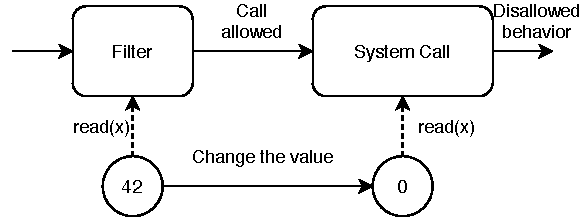
\includegraphics[width=.85\linewidth]{img/tocttou.pdf}
  \caption{Bypassing a system call filter using a TOCTTOU attack}
  \label{fig:tocttou}
\end{figure}

% \pra{Connect this para to the first point you make before for a smoother transition.}

% Cover the first point
To prevent the change of the accessed memory it is enough to prevent writes to
those location. Considering that the Linux kernel uses a well defined interface
for reading from the user-space (\texttt{copy\_from\_user}), it can be extended
to mark the memory page with the data being read. If those pages are marked as
read-only for the duration of the call, double-fetches are \emph{completely
eliminated}. Even double-fetches exits, both fetches will always read the same
value.

% \nb{Make clearer that you are talking about the new defense mechanism and not
% the actual state of things.}

% Cover the second point. Mention the calls for which it makes no sense to protect
Writes to the marked pages are handled depending on where they come from. Writes
from the kernel go through the well defined interface (\texttt{copy\_to\_user}).
They are saved and executed at the end of the call. This guarantees that all of
the writes from the system call are performed and that the system call executes
correctly. However, a small subset of system-calls (e.g. \texttt{pollfd},
\texttt{futex}) depend on the writes from user-space or double-fetches for the
correct behavior. TikTok must be disabled for such calls.

% Cover the third point
Writes from the user-space will trigger a \emph{page-fault handler} where they
will wait for the unmarking. After the page has been unmarked, the write
instruction will be retried. Threads trying to change arguments still execute
correctly -- they are just delayed.
% \pra{You never talk again about the last two design requirements for a
% double-fetch prevention system. Mention that this mitigation methodology still
% allows for normal executions.}


%\pra{Before stating the contributions, insert a couple of paras detailing how you
%address the problem and then introducing your framework. Then you should give a peek
%into the results of your framework evaluation.}

% Introduce TikTok
We present \emph{TikTok} - a memory marking extension to the Linux kernel. TikTok
provides system-calls with a checkpointed view of the memory at the time they
have been read the first time. This mitigates not only the double-fetch bugs
which can be fixed, but also the bugs which are there by design (e.g., system-call
wrappers). TikTok works on modern Linux distributions (Ubuntu Server 18.04 LTS)
and doesn't require any modifications to user programs.

% Sneak-peek into the results
Benchmarking TikTok showed that multithreaded programs with lots of marking
system-calls, such as Apache, show a 10-15\% drop in performance with TikTok
protecting almost all system-calls. Applications that few protected system calls
show a more modest performance drop (4.5\%), with TikTok having almost no effect
on CPU-intensive programs.
% \pra{Create another para where you give an overview of the results of your evaluation.
% Overhead etc. The actual numbers can be filled in later.}

% Three new things in this paper
The main contributions of this paper are
% \pra{Instead of ordering as framework, technique, technique
% order it as technique, technique, framework as a PoC of the above techniques}:
\begin{itemize}
\item A technique to postpone the writes to marked pages from user-space
\item A technique to defer the writes from the kernel to the marked pages,
      while continuing the execution of the system call
\item TikTok - mitigation for the time-of-check to time-of-use attacks on system 
      call arguments in the Linux kernel
\end{itemize}



%\pra{This seems out of place. Each section would have a lead introducing its purpose
%so this is redundant information.}
%\mat{Each systems paper has the same outline. This paragraph can be removed without loss of information.}
%The rest of the paper is organized as follows: \Cref{sec:background} explains 
%inter-process communication, paging, double-fetch bugs, and the related
%background. \Cref{sec:design} describes how \emph{TikTok} works in theory, while
%\cref{sec:implementation} elaborates on the x86-64 implementation. Related work
%is discussed in \cref{sec:relatedwork}.

% Cover the theory needed to understand how and why TikTok works
% 1) IPC - We need this to argue why the deadlocks are almost impossible
% 2) VM and Page Tables - Why it exists and how it works
% 3) x86 Page Tables - Continue the discussion from the previous section
% 4) Page faults - Explain how and why they happen.
% 5) Copy to/from user - Explain why the API has been introduced
% 6) Double-fetches - Provide a high-level overview
\section{Background}
\label{sec:background}
%\mat{What kind of message do you want to send? Why do we need this background information? Guide the reader in understanding what is necessary and where the problems are.}

% \nb{Section feedback: You introduce a lot of interesting notion. It is however
% not always clear why you need it. It might be interesting to add a bit more
% motivation for each section so that it feels less like a OS book.}
%\pra{Insert lead para giving overview of info presented here as you did in the intro.}
%\pra{In its current state this section looks like an information dump. For each subsection
%in bg give context to the user as to why its relevant for TikTok.}

% \nb{So TikTok affects shared memory,
% message passing uses shared memory and is therefore affected. What is special
% about message passing versus other shared memory usage?}.

% I want to cover why this background is needed. IPC is the most problematic
% because it is used to justify the abscence of deadlocks
\Cref{subsec:ipc} introduces two different ways of communication between
processes - \emph{shared memory} and \emph{message-passing}. TikTok affects both
of these methods because the arguments of the message-passing system calls are
stored in (potentially shared) memory. If TikTok marks message-passing
system-call arguments, this introduces additional synchronization points (waits)
when writing to them. These new waits can interact with already present
synchronization primitives to cause deadlocks. In \cref{sec:deadlocks} it is
explained why this is exceedingly rare.

\Cref{subsec:vm} covers how memory is organized on modern computers and how
permissions are implemented. The virtual memory on x86 processors is described
in \cref{subsec:x86pgtables}, followed by the handling of page faults in
\cref{subsec:pagefaults}. These sections discuss the memory protection
mechanisms used by TikTok.

The API that Linux uses to access the user-space memory and which TikTok extends is
described in \cref{subsec:copy}. \Cref{subsec:doublefetch} details the
double-fetch bugs TikTok is mitigating.

\subsection{Interprocess Communication}
\label{subsec:ipc}

The two main types of communication between processes are \emph{shared memory} 
and \emph{message passing}\cite{silberschatz2018operating}.

% Intro to shared-memory
Shared memory relies on two processes having a section of memory that both can 
access. Data transfer is fast, but the synchronization is problematic. 
Processes must monitor shared memory for changes, leading to unnecessary
polling.

% Intro to message-passing
Message passing consists of one process calling send, and another one calling
receive to fetch the message. Synchronous message passing blocks execution until
the execution of the calls has finished. However, on systems with shared memory
unnecessary copying of messages can occur instead of passing the same buffer to
the receiver.

% The state of the modern OSs and concurrent programs
Modern operating systems support both of these approaches. The downsides are
usually offset by adding the  bare minimum of the other approach (e.g., shared
memory with semaphores, or message passing with shared buffers). Sending
messages and writing to the shared memory at the same time between two processes
is exceptionally rare.

\subsection{Virtual Memory and Page Tables} \label{subsec:vm}

% Introduce the basic terms we use to discuss memory in computers
The operating system (OS) provides an illusion that every process is executing
alone on the processor. To accomplish this, the OS needs to restore the program
state on the context switch between two processes (e.g., CPU registers) and to
prevent processes from accessing each other's memory. Memory is protected by
\emph{virtualization}. Processes use \emph{virtual addresses} that get mapped to
the \emph{physical addresses}. When the OS moves data to a different physical
address, the virtual address referring to the data remains the same. Trying to
read outside the designated virtual memory ranges is forbidden, isolating every
process to its own \emph{virtual memory space}.

% Cover the segmented memory model to show the reader later why today the paged
% memory is being used
Virtual memory can be implemented by storing different processes' data at 
different offsets in physical memory and limiting the access to corresponding 
memory chunks. Each process's memory chunk is called a segment and the 
implementation is called \emph{segmented virtual memory}. The translation is 
accomplished by adding an offset to the virtual address. Considering that 
segments need to be continuous, the free physical memory can be fragmented
such that the OS cannot find a part large enough to store a new process.

\begin{figure}

  \begin{subfigure}[]{.45\linewidth}
    \centering
    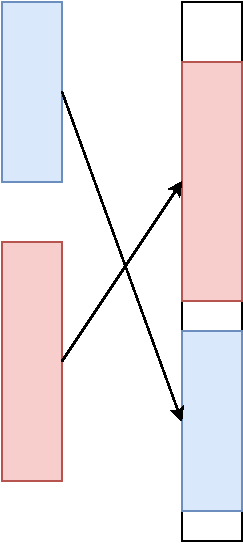
\includegraphics[width=.5\linewidth]{img/segmented.pdf}
    \caption{Segmented}
  \end{subfigure}
  \hfill
  \begin{subfigure}[]{.45\linewidth}
    \centering
    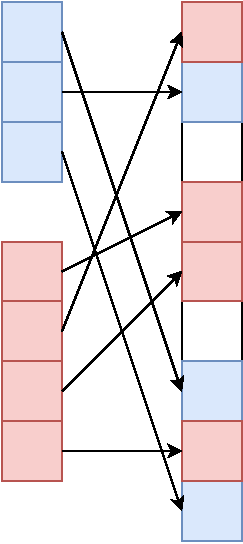
\includegraphics[width=.5\linewidth]{img/paged.pdf}
    \caption{Paged}
  \end{subfigure}

  \caption{Two virtual memory spaces mapped to physical memory using segmented
  and paged approaches}
\end{figure}

% Paged VM and the introduction to permissions we will later use in TikTok
\emph{Paged virtual memory} is more flexible. The physical memory is partitioned
into fixed-size pages (usually 4 kB). A page in the virtual memory space gets
mapped to the corresponding page in the physical memory. The mapping function is
defined for each process by a \emph{page-table}. Page-tables store the reference
to the mapped physical memory (\emph{page frame}). They also keep the access
permissions for each page (\emph{read}, \emph{write}, \emph{execute},
\emph{user}, \emph{superuser}). In case of low memory, rarely accessed pages can
be moved to the disk, and replaced by immediately needed pages. This process is
called \emph{swapping}. Similarly, when processing a file, pages do not need to
be loaded immediately, but only on the first access (\emph{on-demand paging}).
The \emph{present} bit is added to differentiate between present and absent
pages.

% INtroduce page-tables and the TLB
Virtual memory spaces are quite large ($2^{64}$ bytes on a 64-bit processor). A
table containing all one-to-one mappings would be impossibly large to store.
Page tables are therefore stored as trees with only the allocated memory being
present (\cref{fig:pagetable}). However, instead of just reading the
corresponding physical address on memory access, the processor now needs to
perform a tree traversal. Different bits in a virtual address encode the path
the processor needs to take to obtain the page frame number (e.g., the first
eight bits tell CPU which entry on the first level it needs to dereference).
Traversal needs to be fast. It is implemented in hardware by the \emph{memory
management unit} (MMU). Reading the page table from memory is slow, so a small
cache --- \emph{translation-lookaside buffer} (TLB) --- is added to the MMU to
store frequently accessed page entries. On modern processors, a TLB consists of
several levels, and can even be backed by another MMU cache. 
% \nb{Good paragraph!}

\subsection{x86-64 Page Tables}
\label{subsec:x86pgtables}
\begin{figure}[]
  \centering
  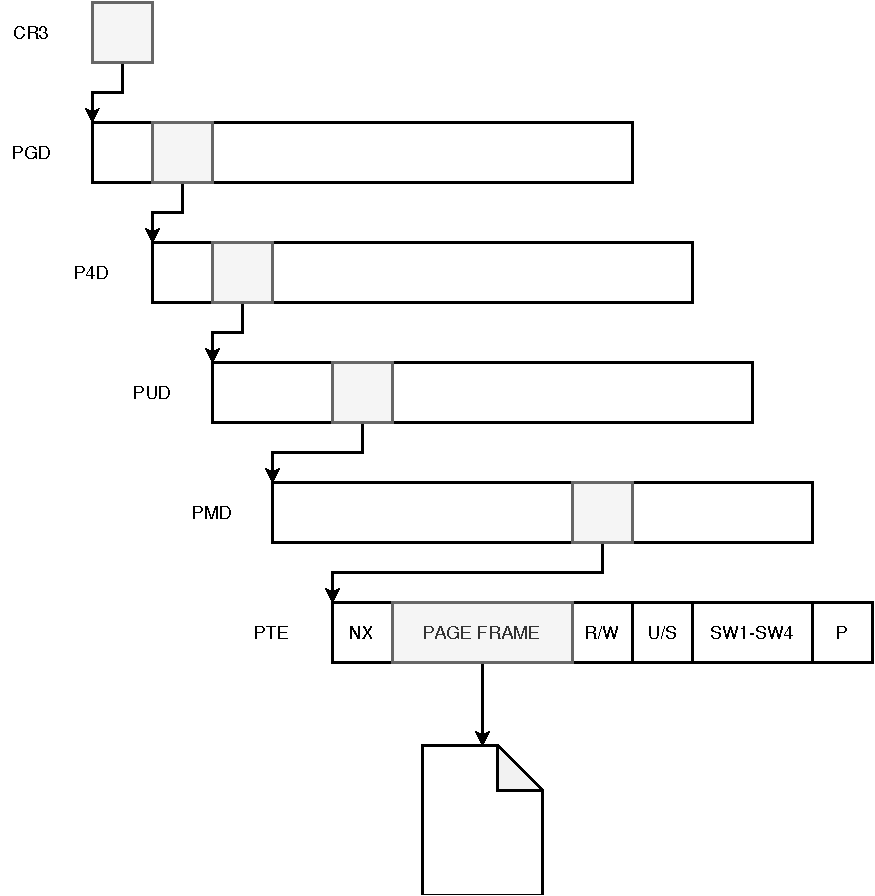
\includegraphics[width = .35 \textwidth]{img/pagetable.pdf}
  \caption{Page Table Structure on x86. Only relevant data has been included.}
  \label{fig:pagetable}
\end{figure}
x86-64 architecture officially supports paged virtual memory model with a 5 
level page table (\cref{fig:pagetable}):
%\nb{indentation looks a bit weird}
\begin{description}
    \item[PGD] Page Global Directory
    \item[P4D] Page Fourth-level Directory
    \item[PUD] Page Upper Directory
    \item[PMD] Page Middle Directory
    \item[PTE] Page Table Entry
\end{description}

% The flags are needed to discuss marking
Every level corresponds to eight bits in the virtual address, with the remaining twelve
bits identifying the offset in the actual page frame. A page table entry
includes the following information:
\begin{description}
    \item[Present bit (\textbf{P})] is set if the page is present in memory
    \item[Read/Write bit (\textbf{R/W})] denotes if the page is writable or just
         readable
    \item[User/Superuser bit (\textbf{U/S})] represents if the page can be 
    accessed by the user, or only by the superuser
    \item[Not Executable bit (\textbf{NX})] is set if the code stored on the 
    page cannot be executed
    \item[Page Frame Number] denotes the page frame the entry points to
    \item[\textbf{SW1-SW4}] Four bits free for the OS to use
\end{description}

\subsection{Page-Faults}
\label{subsec:pagefaults}
% Explain what a page fault is, as well as COW (mentioned later as an optimizaiton)
On an invalid access (e.g., wrong permissions, page not present) the MMU will
trigger a page-fault. The fault is a synchronous interrupt that executes in the
context of the faulting (accessing) thread. The page-fault handler loads an
absent page from the disk. In the case of a write to a temporarily shared page,
it creates an independent, separate copy of the page (\emph{copy-on-write}). On
permission violation, the page-fault handler kills the thread. After the fault
finishes executing, the faulting instruction is re-executed. 

% Later in the paper we require the administrator to disable user-space
% page-fault handling
With the advent of cloud computing, \emph{user-space page-fault handling} has
been added to the Linux kernel. Users can define their routines to load
swapped-out data. This is particularly useful on computer farms when migrating
virtual machines between physical nodes. One only needs to migrate the code that
is executing. Accesses to the unmigrated memory will be passed to the user-space
page-fault handler. It will then fetch them over the network and continue the
execution.

\subsection{Anonymous and File-Backed Pages}
\label{subsec:anofilepages}

Memory in Linux can be either \emph{file-backed} or? \emph{anonymous}.
File-backed pages have a map to the corresponding file. Anonymous pages do not
have a backing file (e.g., stack and heap).

Another classification is based on privacy: \emph{private} and \emph{shared}. 
Private memory is part of only one virtual memory space. This memory space can 
be accessed by multiple threads in a process, but no threads outside the process
have access. Shared memory can be accessed by multiple processes.

% This is the most important paragraph and a basis for one of the attacks. The
% previous two paragraphs are just the introduction
Unlike private memory and shared anonymous memory, shared file-backed memory can
be mapped and unmapped at will. Its content is backed by a file, so the data is 
preserved between (un)mappings.

% \begin{table}[]
%   \begin{tabular}{|l|l|l|}
%   \hline
%           & Anonymous         & File-backed                           \\ \hline
%     Private & /                  & Copy-on-write                         \\ \hline
%     Shared  & Inherited by fork & Can be (un)mapped at any time         \\ \hline
%   \end{tabular}
% \nb{better sign than better sign than /}
%   \caption{Properties of the different types of memory in Linux}
%   \label{tab:memory}
% \end{table}



\subsection{Copy-from-User and Copy-to-User}
\label{subsec:copy}
% Explain the invariants for the addresses in Linux
Linux uses swapping only for user memory. When executing in the kernel context,
kernel memory is mapped and present. A page fault on kernel memory access is
therefore considered fatal. However, the kernel needs to access potentially
paged-out user memory. The user memory is also limited to the lower half of the
virtual memory space. On every access to the user-pointer, the kernel needs to
verify this constraint.
% \nb{just to make sure: constraint = lower half of memoryspace?} Yes

% Move the checks for variants into a separate API
Linux provides functions and macros for user-memory access from the kernel to 
enforce the checks. A page-fault generated by them is treated as a fault in the
user process which had invoked the executing system call.

%\pra{This looks very space inefficient formatting.
%Tabular environment or just in plaintex would conserve more space.}:

% List the API functions
The interface for communication with user-space: \texttt{(\_\_)copy\_(from/to)\_user},
\texttt{(\_\_)(get/put)\_user}, \texttt{user\_str(cpy/len)}.
BSD also provides a similar interface using \texttt{copy\_in} and 
\texttt{copy\_out} functions.

\subsection{Double Fetch Bugs}
\label{subsec:doublefetch}

\begin{figure}[]
  \centering
  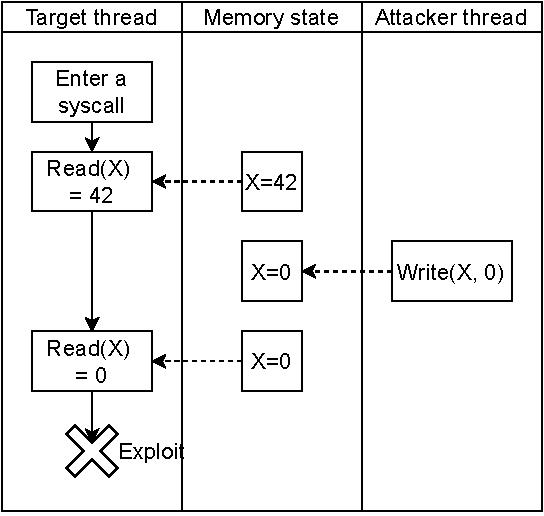
\includegraphics[width=.85\linewidth]{img/doublefetch.pdf}
  \caption{Diagram of a double-fetch bug}
  \label{fig:doublefetch}
\end{figure}

% The idea behind double-fetch bugs
\emph{Double-fetch} bugs occur when a privileged environment (such as the
kernel) reads untrusted memory two or more times and the read values aren't
identical. (\cref{fig:doublefetch}) In between those two reads, memory could
have been changed by an unprivileged adversary. Considering that this bug relies
on carefully timed accesses for two different threads, it is a variant of a race
condition. The situation where the first fetch validates the value of the
fetched variable, but the computation is only performed on the second fetch, is
called a \emph{time-of-check to time-of-use} (TOCTTOU) bug. TOCTTOU bugs have
been widely studied in file systems, where the API makes it possible to swap the
file after validating the access rights \cite{payer2012protecting,
pu2006methodical, wei2010modeling, tsafrir2008portably}.

% Double-fetches are actually so big that people have actualy spent time
% to study them
Wang et al. explain in \cite{wang2018survey} that double-fetches appear not only
in kernels, but wherever there is a trust boundary to cross (e.g., kernel ---
hypervisor\cite{wilhelm2016xenpwn} and hardware --- kernel
boundaries\cite{lu2018untrusted}). Double-fetches have been responsible for many
vulnerabilities in different kernels\cite{jurczyk2013bochspwn, wang2018survey}.

% Explain generally how TikTok works. We mention all the problems that
% TikTok needs to mitigate: writes from user-space, writes from the kernel, safely
% stopping the writes, preventing bypass using file-backed pages, system calls
% that are ignored. The most important part is showing the conditions for 
% introducing deadlocks
\section{Design}
\label{sec:design}

\subsection{The Security Model}
\label{subsec:secmodel}
%\nb{Wouldn't it make sense to introduce the security model before the attacks?}

% Define the power of the adiministrator
The administrator has set up \emph{Discretionary Access Control} (\emph{DAC})
that can prevent the adversary from accessing certain files. They also control
which file-systems are mounted on the machine and have disabled user-space
page-fault handling. 

% Explain why they need every piece of the jigsaw
TikTok relies on the page-fault handler to protect the system. User-space
page-fault handling would enable the malicious user to bypass it completely.
Some files, or even entire file-systems, may change in real-time (e.g. devices
or \texttt{/proc}) bypassing TikTok. DAC or dismounting can be used to prevent
the malicious user from accessing them.
% \nb{It is not really clear to me what these restrictions mean. A few sentences
% explaining what are the consequences of disabling user-space page-fault handling
% might help for example.}

% How does the adversary win the game?
The malicious user has access to a user account on a target machine. They can
execute arbitrary code (including system-calls) and want to obtain root access
by triggering a TOCTTOU bug in the kernel.

%\pra{This section does not really look like a "high-level overview" but more like
%the detailed design itself. :) I would suggest having a separate overview subsection that summarizes
%the main design points.}
%\mat{Style: don't write 'in this section'. It's obvious that it's in this section, so you're just wasting space.}

%\pra{A general comment on the design. Currently, it reads more like a tutorial about
%a cool framework rather than an actual design. All the necessary information required to
%create a design section is here, it just needs to presented better and in a more structured
%way.:) 
%As a suggestion, I think in this section you should first enumerate all possible attack vectors
%for an adversary trying to mount a toctou attack and then present your design policies(3.2, 3.3, 3.5 and 3.6) and
%how they address those attack vectors. IMO the deadlock issue (3.4 and 3.7) is something that 
%needs to be discussed separately since it is not a part of your actual design but moreso
%a consequence of your design.}
%\mat{Agreed with Prashast}
\subsection{Overview}
\label{subsec:designoverview}
% \nb{The paragraphs in this section don't flow really well.}

% Give the bare-bones intro to the attacks
TikTok protects the pages storing the system-call arguments by marking them
read-only. The capabilities of the attacker trying to bypass these measures
are described in \cref{subsec:secmodel}.

% \nb{I would introduce a bit more which attack is about, how they can take place,
% and clearly define what is correct behaviour.}

% List the attacks and explain every one in detail
TikTok needs to protect the arguments from different types of attacks:

\begin{enumerate}
  \item \label{first} Writes from user-space
  \item \label{second} Writes from the kernel
  \item \label{third} Bypassing TikTok by mapping file-backed pages as writable
  \item \label{fourth} Bypassing TikTok by using a write call
  \item \label{fifth} Bypassing TikTok by mapping device-backed files
\end{enumerate}

\emph{Writes from user-space} consist of a malicious user trying to directly
write to the argument stored in memory, while the system-call is being executed
in another thread. The system-call should be unaffected, but the write should
still be performed.

\emph{Writes from the kernel} are indirectly triggered. The user performs a \texttt{read}
system-call with the target address as the destination. The data is then written
to this location by the \texttt{read} system-call with the kernel privileges.

\emph{Bypassing TikTok by mapping file-backed pages as writable} is accomplished
by mapping marked pages in another process. The user stores the arguments on a
file-backed page and maps the file as writable while the system call is executing.
They are then free to write to the marked arguments.

\emph{Bypassing TikTok by using a write call} is accomplished by calling a
\texttt{write} system-call on a file with arguments. Even though the arguments
cannot be changed by directly writing to them, it may be possible to bypass it
by executing a \texttt{write} call.

\emph{Bypassing TikTok by mapping device-backed files} depends on devices
changing the values of their registers independently of writes. Arguments stored
in such a memory region change their values based on the state of the underlying
hardware. File-systems which report the state of the OS (\texttt{\textbackslash
proc}) also belong in this category.

% Give credit where due, but also highlight how difficult this problem is
All of these potential vulnerabilities have been noticed by
Watson\footnote{User-space and kernel writes were not differentiated between}
when he analyzed CerbNG\cite{watson2007exploiting} and other system call
wrappers. TikTok must ensure that the protections don't interfere with the
correct execution of the kernel and user programs. In other words - both writes
and the execution flow can only be temporarily affected.

% Simple solutions don't work
The paradox of memory marking schemes can be seen in the case of system calls
that both read and write to the user memory (e.g., \texttt{rt\_sigaction}).
Simply marking the pages as read-only prevents attacks from the user-space, but
also stops the system call from performing the required write. However, if one
enables the writes for the kernel, the adversary can bypass the protection
using a simple \texttt{sys\_read} call to the marked page.

The protection against the attacks \ref{first} and \ref{second} are described in
\cref{subsec:memorywrites}. The defenses against \ref{third}, \ref{fourth}, and
\ref{fifth} are discussed in \cref{subsec:filewrites}.
%\nb{Kernel writes have their own section now.}
% N.B.Kernel and User-space writes have their own separates section.
% U.T. They are in a single section.


\subsection{System Call Argument Protection}

% \nb{What's the point of the colored arrows in the Figures?}
% U.T. I WILL NEED TO ADD A LEGEND. GREEN - BRANCH YES; RED - BRANCH NO

\label{subsec:memorywrites}
\begin{figure}[]
  \centering
  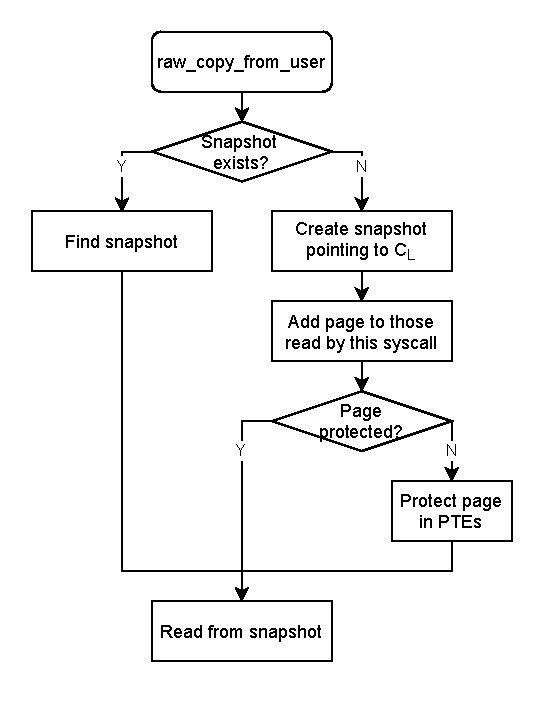
\includegraphics[width = .45 \textwidth]{img/copy_from_user.pdf}
  \caption{\texttt{copy\_from\_user} marks both the file and the pages before
  reading in the data}
  \label{fig:copyfromuser}
\end{figure}

%\pra{I think 3.2 and 3.3 can be merged together into something named along the
%lines of "System Call Argument protection" subsection. The lead for this merged
%section should use threat model as motivation to show that syscall arugments can
%be manipulated from both user and kernel space by adversary. Then, you should
%detail how TikTok handles them as explained below.}
% \nb{I don't remember you introducing memory spaces} 
Defending against the writes from user-space (\cref{first}) is the primary
feature of TikTok. System calls read user memory using \texttt{copy\_from\_user}
and its variants. Calls to \texttt{copy\_from\_user} mark the pages as
\emph{read-only} in all virtual memory spaces mapping it (\cref{fig:copyfromuser}). Multiple system
calls can mark a page at the same time. The benefit of marking the page this way
is that it can still be read by other user threads, reducing the performance
penalty of TikTok. When all the system calls that use the page finish executing,
the page is \emph{unmarked} --- the previous permissions are restored.

However, marking the pages is the first part. TikTok needs to guarantee that the
programs still execute correctly. User-space writes to the marked pages trigger
a page-fault (\cref{fig:pagefault}). In the page-fault handler TikTok intercepts
these writes and stops them until the page has been unmarked. After the
unmarking, the thread will exit the handler and redo the write. This technique
introduces additional synchronization points for concurrent programs. Combined
with the coarse granularity of pages (4KBs) deadlocks come up as a potential
problem. During the evaluation of our system we haven't encountered any
deadlocks due to the new synchronization points. The reasoning behind their
scarcity is discussed in \cref{sec:deadlocks}.
% \nb{This seems quite pessimistic. You might want to put a bit more optimism
% here.}

\begin{figure}[]
  \centering
  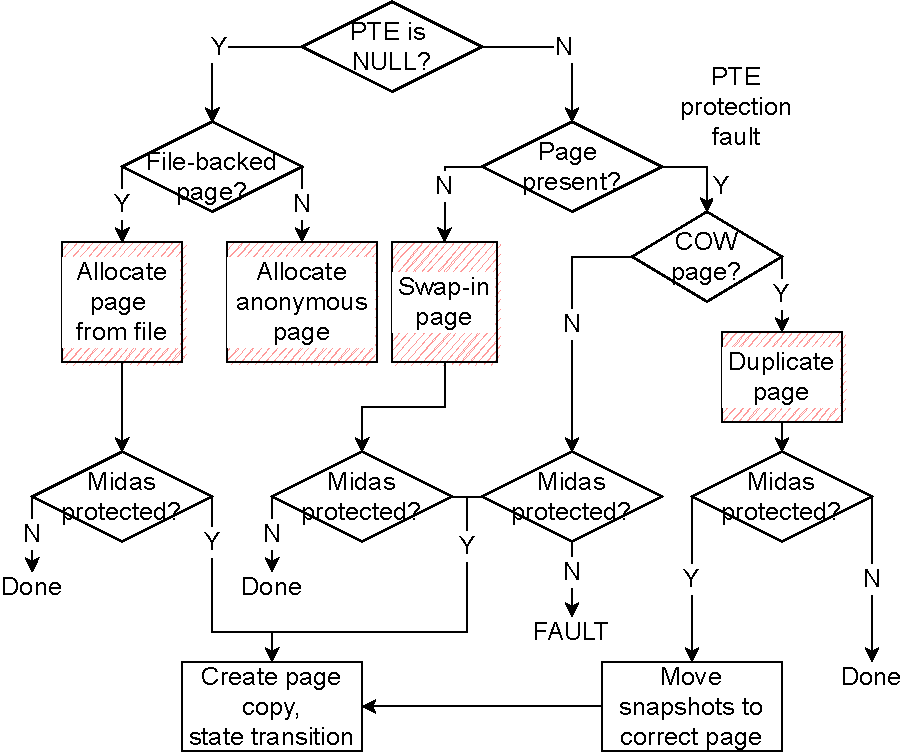
\includegraphics[width = .75 \linewidth]{img/pagefault.pdf}
  \caption{TikTok's handling of the writes to a marked page}
  \label{fig:pagefault}
\end{figure}

\subsection{Protecting System Call Arguments from Writes by the Kernel}
\label{subsec:kernelland}
\begin{figure}[]
  \centering
  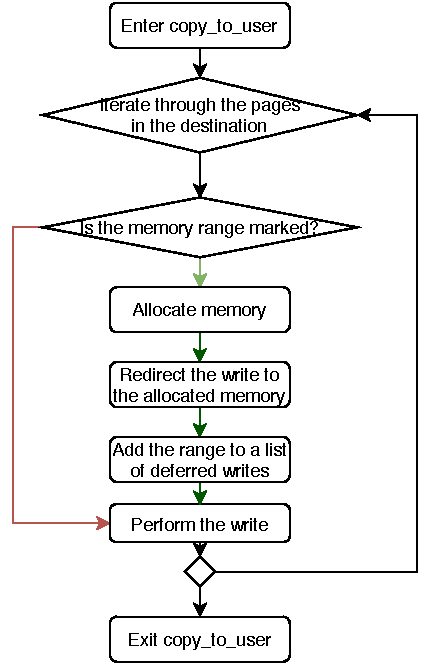
\includegraphics[width = .30 \textwidth]{img/copy_to_user.pdf}
  \caption{\texttt{copy\_to\_user} defers the writes from kernel until the end
  of the system call}
  \label{fig:copytouser}
\end{figure}

% \nb{not absolutely clear why it's
% self-deadlock. You assume read -> block page -> write can't execute?}

The process that stops the user-space writes cannot be applied to the writes
from the kernel (attack \ref{second}). As mentioned in
\cref{subsec:designoverview}, such a system would self-deadlock after a system
call performs a read, mark an argument and a write to the same argument or page
(\texttt{rt\_sigaction}). Any solution involving giving the write permissions to
the kernel results in the adversary bypassing the marking using a system call
(e.g., \texttt{sys\_read}).

Unlike user-space writes to user memory, which can happen from any place in the
code, kernel writes can only take place from \texttt{copy\_to\_user} and its
variants. TikTok uses this to its advantage. When the kernel uses
\texttt{copy\_to\_user} to write to a marked page the write is \emph{deferred}
until the end of the call. The function \texttt{copy\_to\_user} exits normally
with the data saved into a data structure. This prevents self-deadlocks because
the program continues the normal execution. At the end of the call (\emph{after
unmarking}), the writes are performed from the data structure in the order in
which they arrived. If the pages are still marked, the writes will wait just
like the writes from the user-space.

These two techniques create a snapshot of the memory at the moment it
was accessed for the first time. This means that all reads will always return
the original values, even if a call had written to them in-between. In case a
system call performs a re-read of the location it has written to and expects a
new value, TikTok would return the old one. However, the authors haven't
encountered such a case, and TikTok can be easily extended to support it. 
%\nb{By handling this edge case particularly or is there a more general approach?}
% To support this edge case. It is a matter of philosophy. Currently we have a
% have a memory snapshot. One can argue that the edge-case is a double-fetch bug.
% Writing to user-space and reading the same information back is quite strange.
% The fix would just involve checking if the location we want to read from has 
% already been written to. The written data would then be returned instead of 
% the data currently in RAM.

%\nb{The two following paragraph are a bit messy.}
Some system-calls rely on writes from user-space to user-space memory for their
correct behavior. During the execution of these calls the memory is changed and
re-read by the kernel. Hence, memory snapshotting is detrimental to these calls.
Changing the value of the arguments for these calls isn't an attack --- it is a
part of their functionality.

The best representatives are \texttt{pollfd}\cite{pollfd} and
\texttt{futex}\cite{futex}. \texttt{pollfd} checks if any of the
file-descriptors in the array passed as an argument are ready to perform I/O.
The user can write \texttt{-1} to memory to indicate that the loop in the call
needs to skip the descriptor. \texttt{futex} is a user-space mutex. Most of
\texttt{futex} synchronization depends on atomic user-space writes, with the
system-call being performed only to awake or make threads wait. If
\texttt{futex} marks a user-space address as read-only, other user-space threads
will be incapable of unlocking the futex by writing to that address. Adding
these calls and their variants to the exception list lead to a successful boot
and functioning of the kernel in the prototype.

% \nb{So your tool cannot
% protect every system call? This information was not laid out beforehand which is
% a bit surprising.}
% I've split the previous paragraph in two and added a reference to these calls
% to the introduction

%\nb{Hmm, you are ignoring
%even more calls without precising which one. I'm slowly starting to think that
%your system is only working for a few ones that you manually picked...}
%
% IT IS TRUE! I AM A FRAUD :'( Write still works if being protected. It is just
% slower.

The administrator can also choose to ignore certain calls to achieve better
performance. However, this can be applied only to some calls. The arguments
stored in memory need to be \emph{unformatted} --- their content isn't important
for filtering. For such a system-call the TOCTTOU attack would be equivalent to executing
a system-call with the new arguments. An example of such a call is
\texttt{write}. However, in the rare case that a filter in system-call wrapper
needs to prevent a certain string from being written into a file, such
optimizations would need to be disabled. This optimization doesn't enable the
call to bypass TikTok. Even though its arguments aren't marked, it isn't allowed
to write to the marked arguments of other calls.In the future integrating TikTok
with eBPF would enable fine tuning of which system-calls and wrappers are
protected from double-fetches.


\subsection{Protecting Against File-Based Attacks}
\label{subsec:filewrites}
% \nb{This sound really similar in style to the background info from earlier}

A malicious user can bypass memory-marking protections by executing the following
sequence (Attack \ref{third}):

\begin{enumerate}
  \item Map a file \texttt{F} in the process \texttt{A} to a page \texttt{P}
  \item Execute a system-call with the arguments placed on \texttt{P}
  \item The first fetch in the system-call occurs
  \item Map the file \texttt{F} as writable in the process \texttt{B}
  \item Change the values of the arguments on \texttt{P}
  \item The second fetch in the system-call occurs
\end{enumerate}

% \nb{I'll need a bit more info to understand this
% attack. You have a shared+filebacked memory that is used in a double fetch, then
% what happens?}
% \nb{The following sentence is not clear. What does "check"
% means? Mark them as read only?}
% \nb{You can reiterate what is the effect and why
% it is useful.}


To prevent the attack TikTok checks when mapping a new file-backed page if
it is already marked. Such pages are then mapped as marked in the second process
as well.

% \nb{What does it has to do with the previous paragraph? You just gave us a
% solution to our problem and reintroduce new concepts.}
However, another attack may be possible on systems with shared memory and file buffers.
Files in Linux can be accessed in two ways:
\begin{itemize}
    \item by mapping the file to memory
    \item by using system calls to modify the file (e.g., \texttt{write})
\end{itemize}

% \nb{Ok, so that was to introduce the next attack. Either do it in word, "Attack
% 3 is concerned with files access which can be done in two ways in Linux" or
% start a new section.}
Watson\cite{watson2007exploiting} has noticed that protected file-backed pages
could still be edited by a \texttt{write} call if the system uses the same pages
for memory-mapping and buffering when communicating with the block-devices
(Attack \ref{fourth}). The mapped memory would then reflect the state of the
file changed by the \texttt{write} system-call. TikTok prevents this attacks by
pausing the write to the corresponding file as long as it has any marked mapped
pages. As in the \Cref{subsec:memorywrites} no deadlocks were encountered during
testing and the reasoning is discussed in \Cref{sec:deadlocks}. 
% \nb{Third time speaking about deadlock. You might want to
% mention early on that it's not too big of a problem. I'm getting worried the
% whole paper I'm reading will come up with a 200\% overhead in the end...}

% \nb{Again, transition to the next attack is abrupt. Either new section or at
% least mention where are moving to a new scope.}
Finally, TikTok provides no protection against the Attack \ref{fifth}. TikTok
cannot do anything if the values in the mapped pages can change value
independently of writes (such as devices and other pseduo-files). Considering
that mapping device memory to user-space is considered bad practice, we rely on
\emph{Discretionary Access Control} (\textbf{DAC}) to prevent users from mapping
devices in the first place.
% \nb{So, attack 5 still exists. You might want to mention it in the Design
% overview that you do not protect against all of them.}


\section{TikTok Deadlocks}
\label{sec:deadlocks}

\Cref{sec:design} mentions that TikTok may introduce deadlocks to valid
programs. For an OS extension, even a small chance of a random deadlock violates
the presumption of correctness and is unacceptable. Luckily, TikTok deadlocks
can happen only under specific, rare circumstances which violate the principles
of Interprocess Communication (\cref{subsec:ipc}). Ubuntu Server 18.04 LTS
running TikTok is able to successfully boot and execute programs without
encountering deadlocks.

% \nb{Please be specific on what
% rare means or mention you will lay them out right afterward. The first sentence
% of the next paragraph doesn't reassure me you will not try to bury the deadlock.}

TikTok adds additional synchronization points to multi-threaded programs by
stalling the writes. It is possible for these points to introduce previously
non-existent deadlocks to programs. Such deadlocking threads would need to
communicate using both shared memory (for TikTok to stop one of them) and
synchronous system calls (for TikTok to mark memory).

\begin{figure}
  \centering
  \begin{subfigure}[b]{0.45\linewidth}
  \begin{minipage}{\linewidth}
  \begin{lstlisting}
  1: S(A,T1);  
  \end{lstlisting}
  \end{minipage}
  \caption{Thread 1}
  \end{subfigure}
  \hfill
  \begin{subfigure}[b]{0.45\linewidth}
  \begin{minipage}{\linewidth}
  \begin{lstlisting}
  2: write(A);
  3: unblock_S(T2);
  \end{lstlisting}  
  \end{minipage}
  \caption{Thread 2}
  \end{subfigure}
  \caption{Executing instructions in the specified order causes a deadlock with TikTok}
  \label{fig:deadlock}
\end{figure}


\Cref{fig:deadlock} shows an example of a such communication pattern. Thread 1
enters the system call \texttt{S} and marks a shared page \texttt{A} (\textbf{1}). The
system call \texttt{S} blocks until the corresponding call \texttt{unblock\_S} is called
in Thread 2 (\textbf{3}). While the page \texttt{A} is still marked, Thread 2
attempts to write to it, causing it to wait for \texttt{S} to finish
(\textbf{2}). All of the deadlocking patterns need to exibit a similar combination
of paired blocking calls (\texttt{S}, \texttt{unblock\_S}) with arguments in the shared
memory (page \texttt{A}). Concretely, in \Cref{fig:deadlock}:

\begin{enumerate}
    \item The page \texttt{A} is shared between Thread 1 and Thread 2
    \item Access to page \texttt{A} is not protected by a mutex, or a semaphore
    \item System call \texttt{S} is a blocking system call that receives a 
    signal from another thread
    \item System call \texttt{S} reads its arguments from the page \texttt{A}
    \item Thread 2 needs to write to the same page where the arguments for 
    \texttt{S} are stored (page \texttt{A})
    \item Even though Threads 1 and 2 can communicate using shared memory, 
    Thread 1 needs to also invoke \texttt{S}
\end{enumerate}

Paired, blocking system-calls \texttt{S} and \texttt{unblock\_S} are quite rare
and can be found only in the IPC message-passing and synchronization calls. In
either case, the arguments for those calls need to be stored in shared memory,
instead on the thread's stack. The only synchronization call the authors are
aware of that requires this is \texttt{futex}, which is already ignored.

However, message-passing calls (e.g. \texttt{sendmsg}) can store the data being
sent in shared memory. In that case, the processes are sending using
message-passing the data which is \emph{already available in the shared memory}.

% Having identified the system call \texttt{S}\nb{So only one system call fits the
% bill?}, the conditions for the deadlock
% can be simplified to:

% \begin{itemize}
%   \item Threads 1 and 2 share memory (page \texttt{A})
%   \item Threads 1 and 2 decide to share the data in the shared memory (page
%         \texttt{A}) using message-passing
%       \item Threads 1 and 2 nb{Both? or is one sufficient?}write to the shared memory (page \texttt{A}) during the
%         message-passing call                       
% \end{itemize}

% \nb{Might want to precise what the testing
% was, how long, etc...}
% U.T. Booting with systemd and running Phoronix benchmark (e.g. Apache)

% \nb{Something
% stronger than just a judgement on programming techniques would be great. Was does
% it not make sense?->one type of communication should be sufficient}

Programs usually rely on a single IPC apstraction (shared memory or
message-passing). Even software that uses both of them would do so for separate
functionalities. The program that replicates the communication using both
primitives would be an example of terrible programming practice. During the
testing of TikTok (\cref{sec:evaluation}) on Ubuntu Server 18.04 LTS the system
booted and executed benchmarks without encountering deadlocks.

Similar sequences can be constructed using the write system call protection
presented in \cref{subsec:filewrites}. The same argument can be applied in that
case - the program needs to write to the same data to the file using both memory
mapping and a system call at the same time. We have not encountered such a
problem. I WILL PROBABLY NEED TO RUN UBUNTU FOR 24HRS TO CONFIRM THIS. I DON'T HAVE
ANY STRONGER ARGUMENTS OTHER THAN "IT WORKS FOR NOW". ANOTHER PROBLEM IS IF THERE IS
A LIVELOCK. HOW WILL I KNOW? WHAT PROGRAMS SHOULD I RUN?
% \nb{It seems to me you are dismissing things too quickly. You need to
% make me come to the same conclusion. Additionally, you just added a new possible
% sequence, sure there is no other?}


% Here we mention SOME of the interesting implementation decisions. It is
% mostly related to x86 and should be short. ARM support should also be
% be mentioned, but Future work could be a better section for that
\section{Implementation}
\label{sec:implementation}

%\mat{What's the message here? Say what you implement based on which design decisions.}
TikTok prototype has been implemented on Linux x86-64. However, TikTok can be
ported to any operating systems that use a defined interface for reads and
writes to the user-space, and any architecture that has page tables
encoding access control information. Depending on the available resources
(e.g. the number of free bits in the PTE)
information can be stored in different places (e.g., PTE or global structures).

\Cref{fig:bookkeeping} illustrates some of the most important data structures
used in the prototype --- the PTE with the permissions, the marked page metadata
(number of threads marking the page frame, number of threads waiting for the
unmarking, the reverse mapping information).
% \nb{Might be interesting to reiterate which info we need
% to store}
\Cref{subsec:frameinfo} describes the data about the
physical page frame with some of the limitations due to the need to keep
\texttt{struct page} as small as possible. Considering that one \texttt{struct
page} exists for every page frame on the system, increasing its size would
drastically increase the memory overhead.  The data stored in the page table
(permissions, free bits and page frame number) is explained in more detail in
\cref{subsec:pageinfo}.
%\nb{same as above}
%\nb{Why keep it small?}

\subsection{Storing the Page Frame Information}
\label{subsec:frameinfo}
Linux divides physical memory into page frames. Each page frame is represented
by a \texttt{struct page}. Considering that this structure is replicated
millions of times, every additional field has a tremendous impact on memory
consumption.
\\
\\
To keep the memory consumption low, TikTok uses a single bit in \texttt{struct
page} to mark page frames. Considering that x86-64 has enough bits in the flag
field, we have decided to use one of the flag bits for this purpose.
Architectures that have fewer flag bits (such as x86) can instead use some of
the bits used by other features (e.g., Kernel Shared Memory or NUMA domains). On
\cref{fig:bookkeeping} this field is denoted by \emph{Page Marked Flag}.
\texttt{struct page} also stores a pointer to the \emph{reverse mapping}
information. The reverse mapping is used to find all PTEs \emph{TikTok} needs to
(un)mark.
\\
\\
The marking metadata is stored in a hashmap based on the \emph{page frame
number}. The access to these entries is protected by separate mutexes to improve
the scalability of the system. The metadata comprise the page frame number, the
count of threads marking the page (\emph{owners}), the number of threads waiting
for the page to get unmarked (\emph{guests}), and a \emph{queue} they are
waiting on. 

\subsection{PTE Information}
\label{subsec:pageinfo}

When we mark a page we change some of the flags in the PTEs mapping it
(\cref{fig:bookkeeping}):

\begin{description}
  \item[R/W] gets set to \emph{read-only} to prevent writes to the page
  \item[SW2] gets the old value of \textbf{R/W}
  \item[SW3] gets set to 1 
\end{description}

\textbf{SW2} is used by the Software Dirty Pages
feature of Linux. This feature cannot run alongside TikTok in our prototype.
Other architectures may have less, or more bits available for the OS to use. In
the case of lack of space in the page table, \texttt{SW2} and \texttt{SW3} could
be stored in a separate data structure.

\emph{Copy-on-write} pages have a peculiar optimization. They are marked only in
the process requesting the marking. Writes from other processes will trigger a
copy-on-write mechanism, preventing them from changing the data.

TikTok does a partial flush of the TLB and updates the MMU cache to make these
changes visible immediately. The performance impact of this is analyzed further
in \cref{sec:evaluation}.

\begin{figure}[]
  \centering
  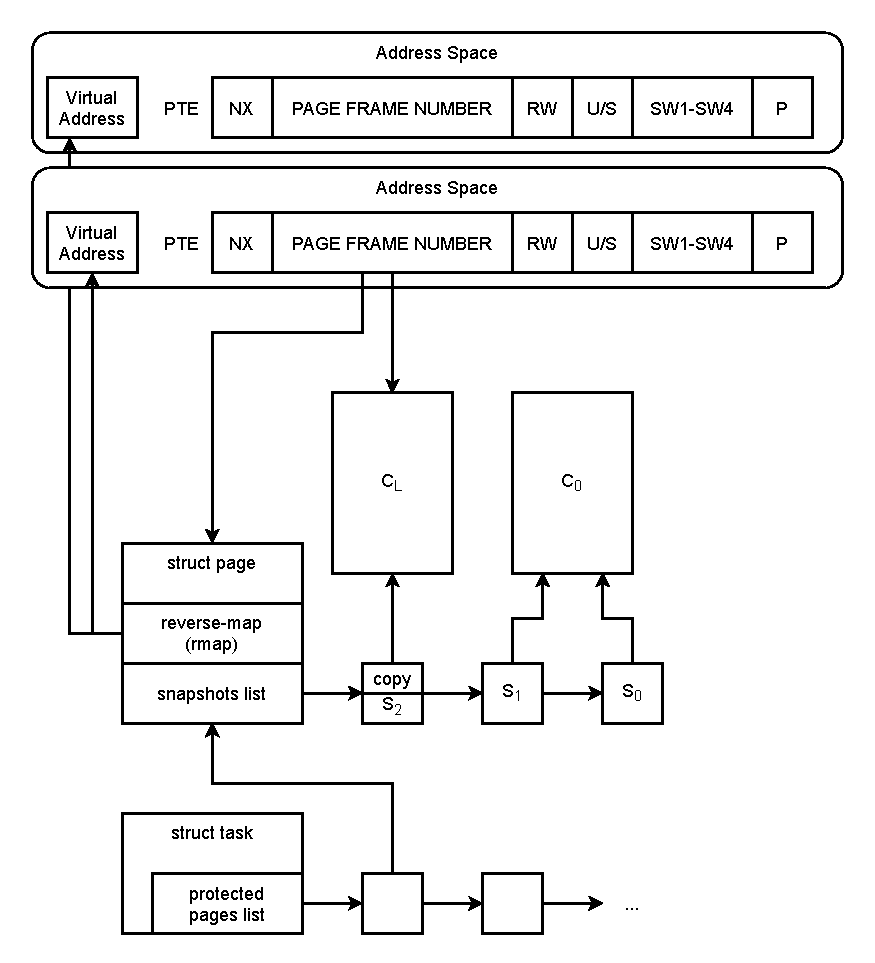
\includegraphics[width=\linewidth]{img/book-keeping.pdf}
  \caption{The most important marking information on x86}
  \label{fig:bookkeeping}
\end{figure}

\section{Evaluation}
\label{sec:evaluation}

\begin{figure*}[]
  \centering
  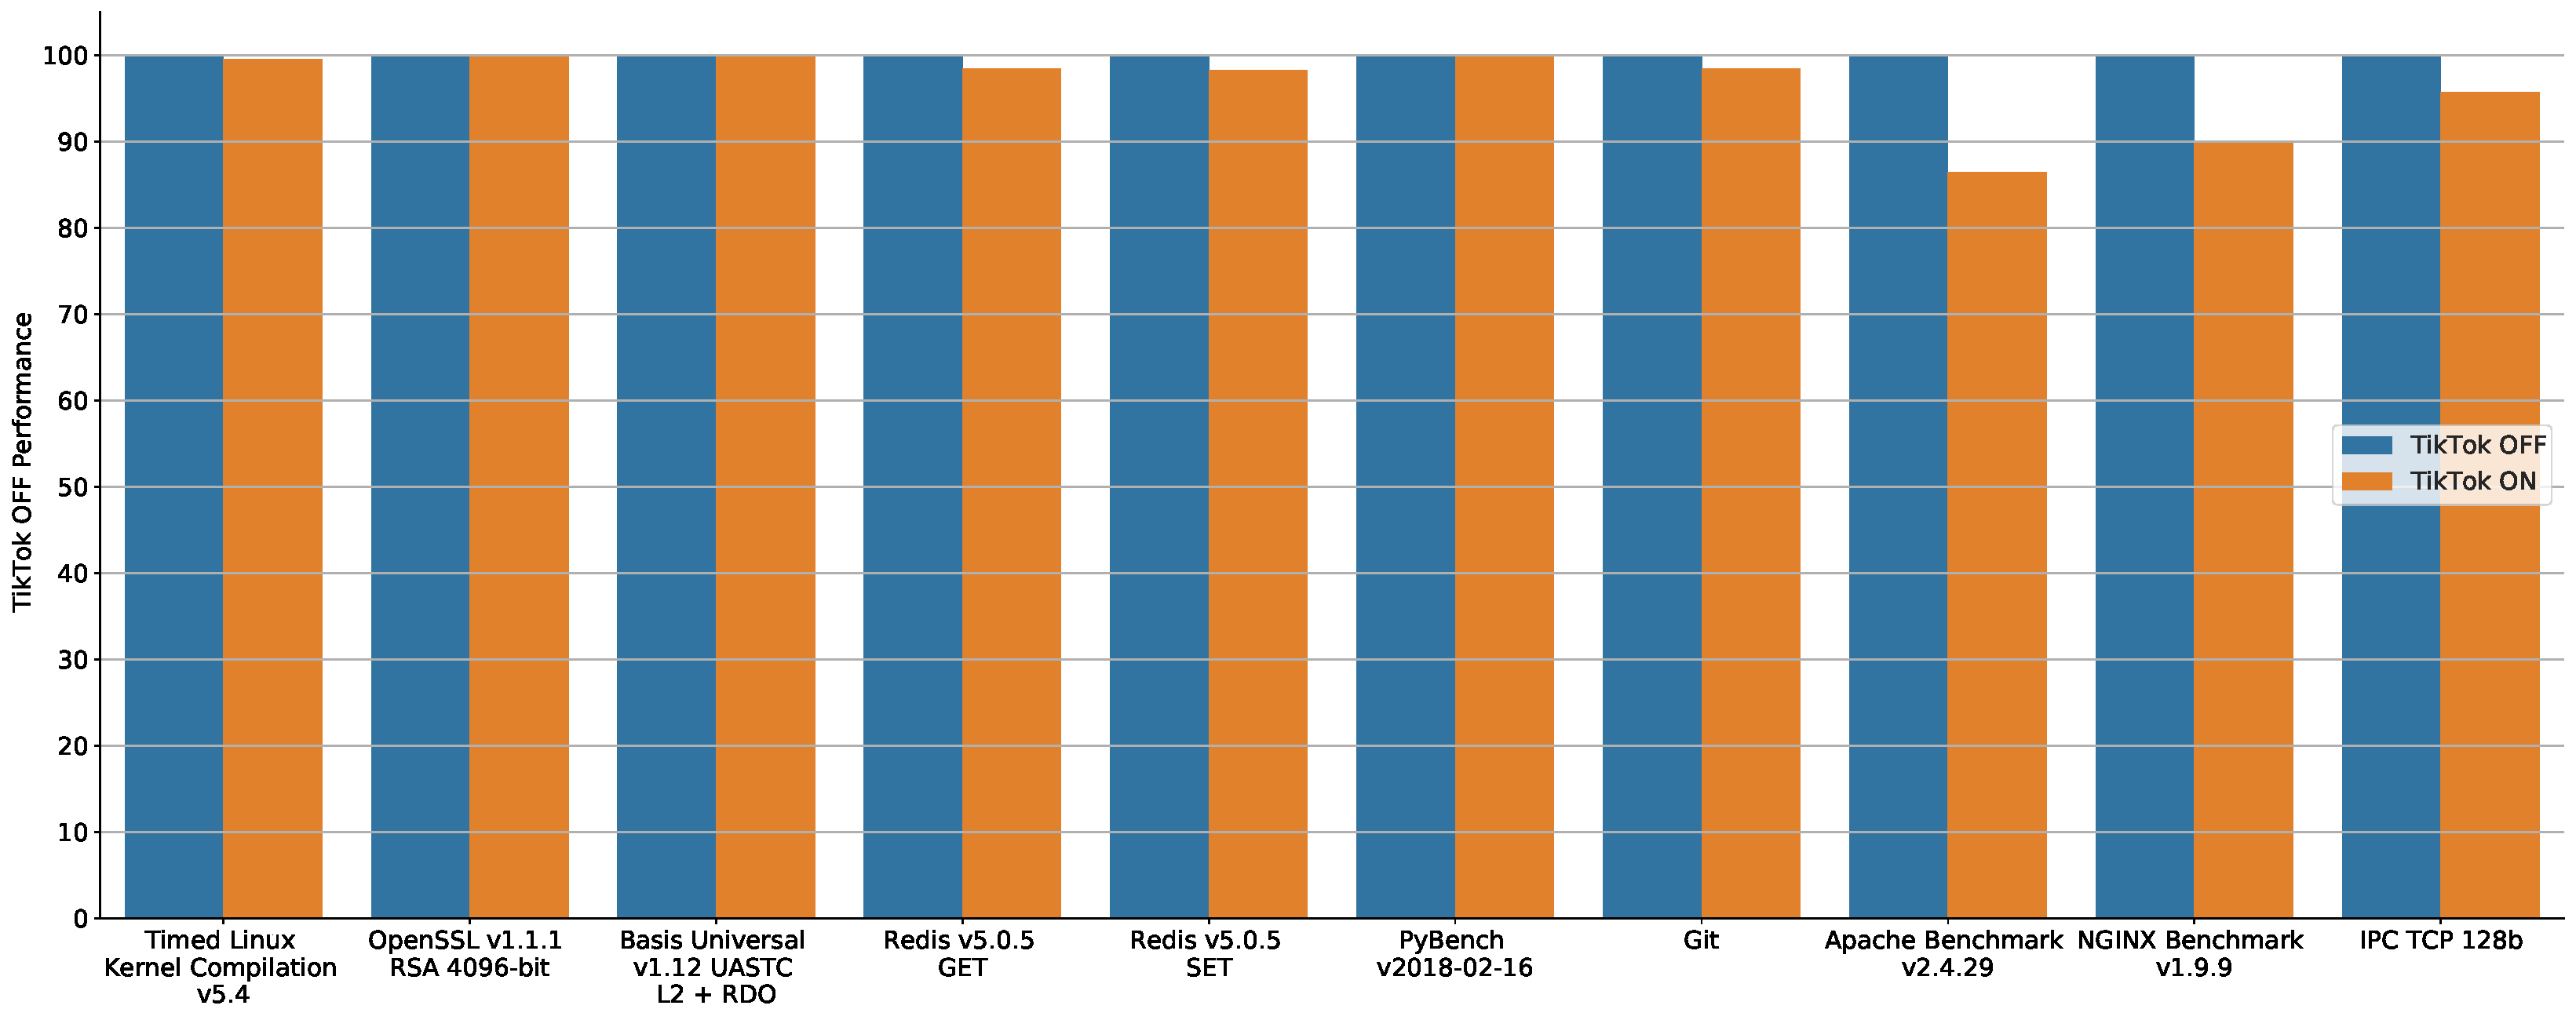
\includegraphics[width=\linewidth]{img/eval.pdf}
  \caption{Performance of TikTok Compared to the Stock Kernel}
  \label{fig:tiktokeval}
\end{figure*}

TikTok has been evaluated on various kernel benchmarks in Phoronix
Test Suite\cite{phoronix}. The test machine was running Ubuntu Server 18.04 LTS
with the Linux kernel 5.4.0-rc3+ on Intel i7-9700 with 16GB of RAM.

\Cref{fig:tiktokeval} shows the results of the Phoronix benchmark. All
results have been normalized to measure performance (higher is better) with the
performance of the stock kernel being the baseline.

Benchmarks Linux compilation, OpenSSL, Redis, Basis, Git and PyBench show a
small degradation in performance --- less than 2\%. These programs don't feature
a lot of inter-process communication. Even the parallelized benchmarks such as
Linux kernel compilation generate independent processes.

However, the two web servers (Apache and NGINX) show a significant drop in
performance (13.6\% and 11.0\%). They are multithreaded applications with a
significant number of system calls being executed. The IPC TCP benchmark has
only two communicating processes and exhibits a smaller overhead (4.3\%).

Analyzing Apache and IPC benchmark executions with \texttt{perf} it was possible
to determine which functions were executing slower with TikTok.
\Cref{table:perf} shows how much time the programs spend in the functions added
by TikTok. Percentages of individual segments have been measured by
\texttt{perf}, while the total overhead is calculated from the results of the
benchmark. Furthermore, TLB is flushed both during the marking and unmarking of
pages.

\begin{table*}[]
  \label{table:perf}
  \centering
  \begin{tabular}{|l|l|l|l|l|}
  \hline
                                 & Apache & Apache (TikTok) & IPC & IPC (TikTok)\\ \hline
  Marking pages read-only        & 0\%    & 4.33\%          & 0\% & 0\%         \\ \hline
  Unmarking pages                & 0\%    & 3.83\%          & 0\% & 0.98\%      \\ \hline
  Flushing Individual TLB Ranges & 1.50\% & 5.72\%          & 0\% & 0\%         \\ \hline
  Write Bypass Protection        & 0\%    & 0\%             & 0\% & 1.47\%      \\ \hline
  Read Bypass Protection         & 0\%    & 0\%             & 0\% & 1.15\%      \\ \hline
  Total Overhead                 & 0\%    & 13.59\%         & 0\% & 4.29\%      \\ \hline
  \end{tabular}
  \caption{Perf Analysis of the Benchmarks}
\end{table*}

The comparison of the Apache and IPC runs shows two very different marking
profiles. Apache spends a considerable amount of time marking and unmarking
pages, while IPC does not mark pages at all. This is a consequence of the
different system-calls used by these applications. IPC uses only \texttt{read}
and \texttt{write} calls which do not mark arguments, while Apache also invokes
system-calls which mark arguments (\texttt{accept}, \texttt{getsockname}).
Consequentially, Apache spends a lot of time marking and unmarking pages.

In these two segments Apache actually waits most of the time for the TLB
signaling functions to execute. \texttt{flush\_tlb\_mm\_range} amounts for
2.51\% (marking) and 2.10\% (unmarking) of the total time spent executing the
benchmark. Frequent TLB flushes are expensive because the CPU needs to make sure
that all the cores have processed the signal before continuing. Unfortunately,
this is only a part of the overhead incurred by flushing the TLB. Flushed pages
will be accessed right afterward leading to a TLB miss, further inflating the
overhead.

IPC benchmark executes only \texttt{write} and \texttt{read} calls. It doesn't
incur any overhead on TLB flushes because none of these calls mark pages.
However, the protections against bypassing TikTok using these calls are still
active, leading to a significant locking overhead. Without TLB flushes it is
interesting to notice that the overhead of individual components roughly adds
up to the total overhead in the IPC benchmark.


% In this section we need to convince the reader in two things:
% 1) Alternative filtering approaches to system call filters are incomplete and
% cumbersome
% 2) The best way to solve the TOCTTOU bug in filters is TikTok. All other
% methods can only fix other double-fetches, or they force you to use TSX
\section{Related Work}
\label{sec:relatedwork}

%\mat{Numbers smaller than 10 should be written out: two!}
The literature related to TikTok can be broadly divided into two groups. In the
first group are system call wrappers whose main vulnerability TikTok is
mitigating. The second ones are the mitigations and solutions for
double-fetches, which are a superclass of TOCTTOU bugs.

We describe the benefits that system call wrappers compared to other solutions.
We show that all other filters that ignore or remove the TOCTTOU problem have
to either reduce the security guarantees they offer, or violate the separation
of the filter and the system call.
% \nb{it could be interesting to mention these
% things beforehand as motivation for tiktok. Otherwise the impostance is not
% obvious to the reader.}

Afterward, we take a look at alternative ways to address the TOCTTOU bug of the
system call wrappers. Most of them are focused on finding and fixing the bug,
which isn't possible in this case. TikTok is also compared against other runtime
mitigations of double-fetches.

\subsection{System Call Wrappers and Filters}

Watson \cite{watson2007exploiting} scrutinized the security of many system call
wrappers. Not only did he found that all of them were insecure, Watson also
described the different types of TOCTTOU bugs and discussed potential fixes. In
a short paragraph, he mentions that Pawel Dawidek, the creator of CerbNG
\cite{zak_frasunek_dawidek}, has experimented with marking arguments read-only.
CerbNG was an early system call filtering system for BSD that used
copy-on-read-and-write to a new memory page.

Afterward, Watson briefly discusses problems such memory marking systems
need to solve: 
\begin{itemize}
    \item unnecessary page-faults
    \item bypassing memory marking using IO system calls
    \item mapping shared memory with different permissions
    \item handling system calls that both read and write to the same memory
\end{itemize}

According to Watson, no memory-marking system (including CerbNG) addressed all
of these problems. TikTok does exactly that. Unnecessary page-faults are rare
and they are used to make the offending threads wait for unmarking. After the
page has been unmarked, the write proceeds without any consequences. Write
system call does not proceed until there are no marked pages of the file. If
needed, pages are marked when they are mapped. TikTok postpones all writes to
marked pages coming from the kernel while allowing the system calls to execute
correctly.
%\nb{Good paragraph!}

Modern system call wrappers can be classified into two groups, based on how they
approach the TOCTTOU attack. The first group eliminates all functionality
vulnerable to the attack. Linux's \emph{SecComp}\cite{seccomp} and
\emph{eBPF}\cite{ebpf} belong to this group. The second group moves the filter
checks deeper into the system calls, eliminating the need to read the arguments
twice. \emph{Landlock Linux} \cite{landlock} and Google's \emph{Kernel Runtime
Security Instrumentation} (KRSI)\cite{krsi} embrace this technique.

\subsubsection{Partial Solutions}
SecComp\cite{seccomp} uses \emph{Berkeley Packet Filter} (BPF) to provide small,
programmable filters that execute before the system call. Based on the values
in registers, Linux can decide whether to allow or to prevent a system call.
However, BPF cannot dereference pointers because an adversary would be able to
bypass those checks using a TOCTTOU attack. \emph{Extended Berkeley Packet
Filter} (eBPF)\cite{ebpf} provides larger filters that can also dereference
user pointers. However, eBPF cannot be used for security purposes --- it cannot
stop system calls from executing. eBPF is completely read-only and can only be
used for tracing.

\subsubsection{LSM-based Solutions}
Landlock\cite{landlock} and KRSI\cite{krsi} use the \emph{Linux Security Module}
\cite{morris2002linux} (LSM) hooks to call filter checks after the arguments
have already been copied into the kernel. LSM hooks have been imagined as a set
of places where arbitrary checks can be performed before accessing a kernel
resource. Execution proceeds only if the execution has been successful.
Different security modules can provide different hooks to provide different
guarantees (e.g., \emph{SELinux}\cite{smalley2001implementing} and
\emph{AppArmor}\cite{gruenbacher2007apparmor}).

Both Landlock and KPSI attach eBPF filters to hooks, allowing users to provide
custom rules for system calls. For this solution to work everywhere for perfect
syscall filtering, LSM hooks would need to be manually added to all Linux
drivers and \texttt{ioctls}. Unfortunately, this is highly impractical and requires
considerable effort from a large group of developers. Considering that LSM
focuses on access control to kernel objects, it is questionable if an LSM module
can be used to mitigate bugs based on the system call arguments. Some of the
bugs could manifest themselves before a hook has been executed. TikTok is a
generic solution that does not require modifying the drivers, nor the use of
LSM hooks. Once it is deployed, all double-fetch bugs are eliminated from all
the drivers. A system call wrapper that uses TikTok can be completely
independent of the implementation of the system calls it is filtering.

\subsection{Double-Fetch Solutions}

Solutions for double-fetch bugs can be divided into \emph{static} and
\emph{dynamic} techniques. Static techniques do not execute the program but
analyze the source code. Dynamic techniques analyze the execution of the
program to find any violations.

\subsubsection{Static Analysis Work}
\label{subsec:dfstatic}
Static analysis techniques analyze the source code to find double-fetch bugs.
Wang et al. \cite{wang2017double} used pattern matching to find potential
double-fetches. They implemented a tool that patches certain double-fetches
automatically. However, their method in the general case produces false
positives that need to be inspected manually. Xu et al.\cite{xu2018precise}
improved on this work by proposing Deadline. Deadline does not use the pattern 
analysis on the source files to detect double-fetches, but a compiler's
intermediate representation and constraint solving to eliminate false positives.

Static analysis techniques such as these have the benefit of being able to find
bugs in the code that we cannot run (e.g., we are missing hardware to test the
drivers). However, they are meant for bug detection, not mitigation. Even though
the tools can fix some bugs automatically, this is not always possible. The
TOCTTOU bug is in system call wrappers by design. Double-fetches not visible in
the source, nor in the intermediate representation are another problem.
Compilers can introduce such invisible double-fetches when allocating registers
to variables. TikTok is a mitigation technique that works even in such cases.


\subsubsection{Dynamic Analysis Work}
Google Project Zero's Bochspwn \cite{jurczyk2013bochspwn} uses an emulator to
detect double-fetches. It found quite a large number of bugs in the Windows
kernel. Bochspwn works on binaries. It does not require access to the source
code and it detects bugs introduced by compilers.
DFTracker\cite{wang2019dftracker} is another dynamic analysis technique work
with a lower overhead, that relies on taint tracking. However, these dynamic
techniques are limited to the detection of double-fetches. Similarly to work
presented in \cref{subsec:dfstatic}, developers need to manually fix the bugs.
However, with dynamic analysis a double-fetch needs to be executed, limiting
this technique to the core kernel and to the drivers with the available
hardware.

A big leap in dynamic analysis techniques has been presented by Schwartz et al.
\cite{schwarz2018automated}. The first part of the paper introduces DECAF - a
framework that uses side-channel attacks to create a fuzzing oracle for
double-fetch bugs. While Bochspwn relies on emulation, slowing the execution
significantly, DECAF runs natively. It also eliminates false positives by
automatically exploiting found bugs.

Schwartz et al. then discuss a real-time mitigation technique for double
fetches - DropIt. DropIt uses Intel's \emph{Transactional Synchronization 
Extensions} (TSX)\cite{intel64and} in a creative way to prevent double-fetch
bugs. By encapsulating the code in a TSX transaction, writes from other threads
to the addresses that have been accessed will result in the
transaction being aborted. However, the code executing inside a TSX transaction
is severely limited. All reads must fit in the L3 cache, and all writes in L1.
Some instructions are also forbidden. TikTok has none of those limitations.
It works on non-Intel processors and relies on page tables for protection - a
technique that has been present for several decades.

\section{Further Work}

Considering the performance impact, it isn't feasable to run TikTok for all
system-calls. Integration with an existing system-call wrapper would lead to the
improved flexibility and performance. SecComp\cite{seccomp} and eBPF\cite{ebpf}
are obvious candidates that would benefit from such an extension. Another
optimization would be to mark only the pages accessed by the filter, and not the
system-call body.

\section{Conclusion}

This work is the first work to mitigate double-fetches in the Linux kernel
without significantly reducing the length and the instructions used in system
calls. In doing so it mitigates a previously unfixable TOCTTOU bug in
system-call wrappers. TikTok also solves the problem the system-call wrappers
have had with system-calls that both read and write into the user-space memory.
These breakthrough make system-call wrappers again a viable solution, not only
for the reduction of the attack surface, but also for the mitigation of
vulnerabilities until a patch is available.
%-------------------------------------------------------------------------------
%\section*{Acknowledgments}
%-------------------------------------------------------------------------------

%-------------------------------------------------------------------------------
\section*{Availability}
%-------------------------------------------------------------------------------

The source code of TikTok is available at LINK. It has been released under the
GNU Public Licence.

%-------------------------------------------------------------------------------
\bibliographystyle{plain}
\bibliography{\jobname}

%%%%%%%%%%%%%%%%%%%%%%%%%%%%%%%%%%%%%%%%%%%%%%%%%%%%%%%%%%%%%%%%%%%%%%%%%%%%%%%%
\end{document}
%%%%%%%%%%%%%%%%%%%%%%%%%%%%%%%%%%%%%%%%%%%%%%%%%%%%%%%%%%%%%%%%%%%%%%%%%%%%%%%%

%%  LocalWords:  endnotes includegraphics fread ptr nobj noindent
%%  LocalWords:  pdflatex acks
